% documentclass
% set font size=11 (11pt)
% set paper format=A4 (a4paper)
% set equation alignment to left (fleqn)
\documentclass[11pt,a4paper,fleqn]{article}


% Preamble
% use the inputenc and fontenc packages to use French accents
\usepackage[utf8]{inputenc}
\usepackage[T1]{fontenc}
% for pseudocolor
\usepackage{algorithm,algpseudocode}
% for code samples
\usepackage{listings}
% for links
\usepackage{hyperref}
% for color
\usepackage{xcolor}
% allow for arbitrary font size
\usepackage{anyfontsize}
% set the font as Time New Roman (the Latex equivalent, at least)
% \usepackage{mathptmx}
% set the size of the document margins using the geometry package
\usepackage[lmargin=0.97in,rmargin=0.97in,tmargin=1.4in,bmargin=1.4in]{geometry}
% turn the color of footnote markers to black
\renewcommand\thefootnote{\textcolor{black}{\arabic{footnote}}}
% suppress indents on footnotes
\usepackage[hang,flushmargin]{footmisc}
% automatically generates colored brackets around references
\usepackage{fncylab} \labelformat{equation}{(#1)}
% supress indent on new paragraphs
\setlength{\parindent}{0pt}
% use the amsmath package to include mathematical symbols
\usepackage{amsmath}
% suppress the space between the left margin and the equations (fleqn still leaves some space by default)
\setlength{\mathindent}{0pt}
% create a new environment to left flush the equation with the align environment
\makeatletter
\newenvironment{lflalign}{ \vspace{-3mm}%
  \def\align@preamble{%
    &\strut@
    \setboxz@h{\@lign$\m@th\displaystyle{####}$}%
    \ifmeasuring@\savefieldlength@\fi
    \set@field
    \hfil
    \tabskip\z@skip
    &\setboxz@h{\@lign$\m@th\displaystyle{{}####}$}%
    \ifmeasuring@\savefieldlength@\fi
    \set@field
    \hfil
    \tabskip\alignsep@
  }
  \flalign}
{\endflalign}
\makeatother
% use the ammssymb package to use mathematical symbols
\usepackage{amssymb}
% create new commands for mathematical symbols
\DeclareMathOperator{\N}{\mathbb{N}}
\DeclareMathOperator{\Z}{\mathbb{Z}}
\DeclareMathOperator{\Q}{\mathbb{Q}}
\DeclareMathOperator{\R}{\mathbb{R}}
\DeclareMathOperator{\Pb}{\mathbb{P}}
% declare the cmsy (computer modern symbol) math alphabet to define appropriate fonts for the U and N mathematical symbols
\DeclareMathAlphabet\mathbcal{OMS}{cmsy}{m}{n}
% create new commands for mathematical symbols
\DeclareMathOperator{\E}{\mathbcal{E}}
\DeclareMathOperator{\Ex}{\mathbb{E}}
\DeclareMathOperator{\F}{\mathbcal{F}}
\DeclareMathOperator{\G}{\mathbcal{G}}
\DeclareMathOperator{\M}{\mathbcal{M}}
\DeclareMathOperator{\HH}{\mathbcal{H}}
\DeclareMathOperator{\QQ}{\mathbcal{Q}}
\DeclareMathOperator{\PP}{\mathbcal{P}}
\DeclareMathOperator{\Noo}{\mathbcal{N}}
\DeclareMathOperator{\U}{\mathbcal{U}}
% use the bbm package to be able to use the double stroke 1 for the indicator function
\usepackage{bbm}
\DeclareMathOperator{\ind}{\mathbbmss{1}}
% use the bm package to use bold characters in math mode
\usepackage{bm}
% create a new command for black square bullets
\newcommand{\bs}{\scalebox{0.7}{$\blacksquare$} \hspace{2mm}}
% use the relsize package to be abe to change the size of mathematical symbols
\usepackage{relsize}
% define a new command for in-line small summation
\newcommand{\ssumm}[2]{\underset{\scriptscriptstyle #1}{\overset{\scriptscriptstyle #2}{\mathlarger{\mathlarger{\mathlarger{\Sigma}}}}} \hspace{0.5mm}}
% define a new command for in-line small products
\newcommand{\sprod}[2]{\underset{\scriptscriptstyle #1}{\overset{\scriptscriptstyle #2}{\mathlarger{\mathlarger{\mathlarger{\Pi}}}}} \hspace{0.5mm}}
% Use the caption package to customize captions (titles) of tables and graphs
\usepackage[font=small,labelfont=bf]{caption}
% use float package to force figure the be positioned where indicated
\usepackage{float}
% use the graphicx package to be able to resize tables
\usepackage{graphicx}


\begin{document}

% command to check unused bibliography entries
% \nocite{*}
{\fontsize{20pt}{22pt}\selectfont \textbf{Probabilistic tools} \par}
\vspace{10mm}
{\fontsize{12pt}{22pt} \textbf{Probabilistic Theory}\par}

\vspace{5mm}

Objectivism: the probability of an event is determined in a unique manner.

\vspace{5mm}

Subjectivism: the probability of an event is not determined in a unique manner.

Bayesianism is a probabilistic theory part of the subjectivism. It states that a probability varies depending on new information (Bayes theorem).

In Bayesian inference, random variables are $X$. $\theta$ is not random and not known. The objective is to estimate $\theta$ using \textit{a-posteriori} probabilities.

\vspace{5mm}
{\fontsize{12pt}{22pt} \textbf{Expectation}\par}

\vspace{5mm}

Generic definition:

$X$ random variable defined on $(\Omega, \mathcal{F} ,\mathbb{P})$:

$\mathbb{E}[X] = \int_{\Omega} X(\omega) d\mathbb{P}(\omega)$

\vspace{5mm}

Using measure theory results, we find the specific cases for discrete and continuous variables.

\vspace{5mm}

For discrete variables :

$\mathbb{E}[X] = \Sigma_i x_i \mathbb{P}(X=x_i)~(= \mathbb{E}_{\mathbb{P}}[X])$

\vspace{5mm}

For continuous variables:

$\mathbb{E}[X] = \int x f(x) dx~(= \mathbb{E}_{\mathbb{P}}[X])$

\vspace{5mm}

Conditional expectation (discrete case):

$\mathbb{E}[Y|X=x] = \Sigma_y y \mathbb{P}(Y=y | X=x)$

\vspace{5mm}
{\fontsize{12pt}{22pt} \textbf{Distribution functions}\par}

\vspace{5mm}

Mass function

The probability mass function (p.m.f.) is the histogram of the distribution, that is:

- x-axis: values

- y-axis: frequency

\vspace{5mm}

Density function

The probability density function (p.d.f.) is the "smooth histogram" of the distribution.

\vspace{5mm}

\begin{center}
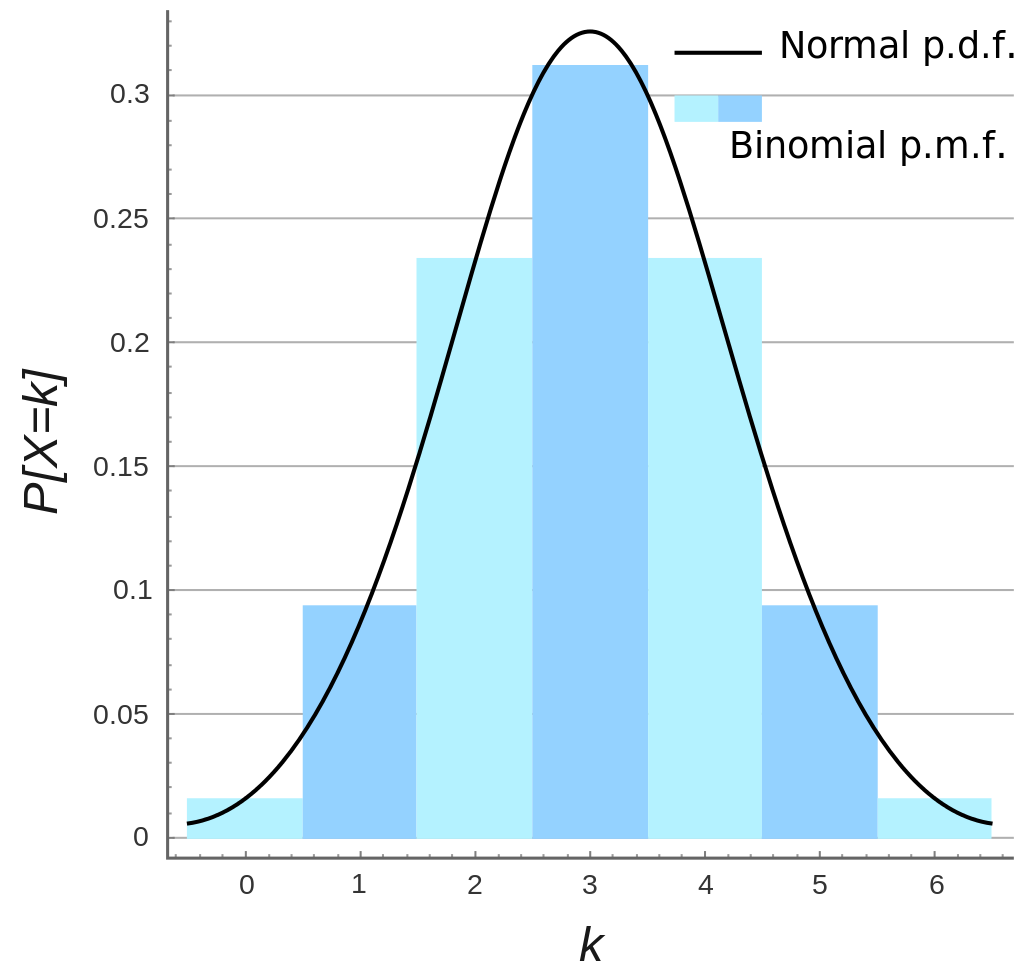
\includegraphics[scale=0.15]{mass_density_functions.png}
\end{center}

\vspace{5mm}

Cumulative distribution function

The cumulative distribution function (c.d.f) is given by $F_X(x)= \mathbb{P}(X < x)$. 

The empirical distribution function is its estimation:
$\widehat{F}_n(x) = \frac{1}{n}\{\text{number of elements} < x\}$

\begin{center}
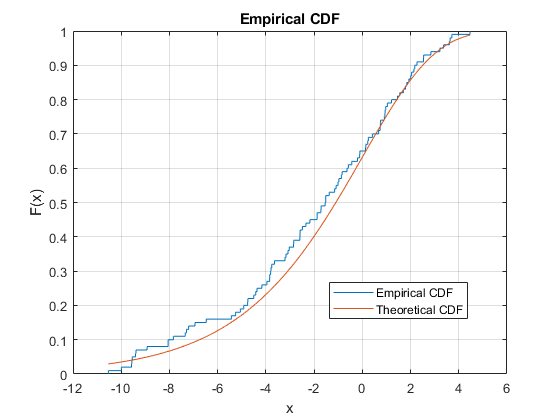
\includegraphics[scale=0.4]{CDF.png}
\end{center}

\vspace{5mm}
{\fontsize{12pt}{22pt} \textbf{Correlation}\par}

\vspace{5mm}

\underline{Pearson coefficient}:

\begin{center}
$\rho_{X,Y} = \frac{cov(X,Y)}{\sigma_X \sigma_Y}$
\end{center}

\textit{np.cov(a,b)} gives a \textbf{matrix} with covariances and \textbf{unbiased} variances (on the diagonal). 

Several computation equivalences are shown below:

\lstset{language=Python}
\lstset{frame=lines}
\lstset{caption={Pearson coefficient replication}}
\lstset{label={lst:code_direct}}
\lstset{basicstyle=\footnotesize}
\begin{lstlisting}

a = pd.Series([5, 2, 6])
b = pd.Series([18, 2, 5])

print(a.corr(b) # biased standard deviation estimators !!
      == np.corrcoef(a,b)[0,1] 
      == (np.cov(a,b)[0,1] / np.sqrt(np.cov(a,b)[0,0]*np.cov(a,b)[1,1]))
      == np.cov(a,b)[0,1] / (np.std(a,ddof=1)*np.std(b,ddof=1)) 
      != np.cov(a,b)[0,1] / (np.std(a)*np.std(b)))

# prints True

\end{lstlisting}

\vspace{5mm}

\textit{Note}: when we compute those statistics numerically, we use \textbf{empirical} values.

Thus, $\mathbb{V}[X] = \mathbb{E}[X-\mathbb{E}[X]]$ is computed as $var_n(x)=\frac{1}{n}\Sigma(x_i - \overline{x})^2$

\vspace{5mm}

\underline{Autocorrelation (1)}:

\begin{center}
$R_{k} = \frac{\mathbb{E}[(X_i-\mu_X)(X_{i+k}-\mu_X)]}{\sigma_X^2}$
\end{center}

$X_i$ is the dataset without the last $k$ values

$X_{i+k}$ is the dataset without the first $k$ values

$\mu_X$ is the mean on \textbf{the whole} dataset $X$

$\sigma_X^2$ is the variance \textbf{the whole} dataset $X$

\vspace{5mm}

\underline{Autocorrelation (2)}:

\begin{center}
$R_{k} = \frac{\mathbb{E}[(X_i-\mu_{X_i})(X_{i+k}-\mu_{X_{i+k}})]}{\sigma_{X_i}\sigma_{X_{i+k}}}$
\end{center}

$X_i$ is the dataset without the last $k$ values

$X_{i+k}$ is the dataset without the first $k$ values

$\mu_{X_i}$ is the mean on dataset $X_i$

$\sigma_{X_i}$ is the standard deviation on dataset $X_i$

\vspace{5mm}

\textit{statsmodels.tsa.stattools.acf} uses formula (1).

\textit{np.autocorr} uses formula (2).

Below is the summary of equivalences:

\lstset{language=Python}
\lstset{frame=lines}
\lstset{caption={Autocorrelation replication}}
\lstset{label={lst:code_direct}}
\lstset{basicstyle=\footnotesize}
\begin{lstlisting}

import statsmodels.tsa.stattools as sm

s = pd.Series([5, 2, 6, 18, 2, 5])

a = pd.Series([5, 2, 6])
b = pd.Series([18, 2, 5])

# Formula (1)
print(s.autocorr(3) # unbiased standard deviation estimators !!
      == a.corr(b)
      ==  np.cov(a,b)[0,1]/(np.std(a,ddof=1)*np.std(b,ddof=1)))

# prints True

# Formula (2)
def acf_by_hand(x, lag):
    y1 = np.array(x[:(len(x)-lag)])
    y2 = np.array(x[lag:])
    sum_product = np.sum((y1-np.mean(x))*(y2-np.mean(x)))
    return sum_product / (len(x) * np.var(x))

print(round(acf_by_hand(s,3),6)
        == round(sm.acf(s)[3],6)) # biased covariance and standard deviation estimators !!

# prints True

\end{lstlisting}

\vspace{5mm}

Below a graphical comparison of both formulas:

\lstset{language=Python}
\lstset{frame=lines}
\lstset{caption={Graphical comparison of correlation computations}}
\lstset{label={lst:code_direct}}
\lstset{basicstyle=\footnotesize}
\begin{lstlisting}

import statsmodels.tsa.stattools as sm

s = pd.Series([5, 2, 6, 18, 2, 5])
a = pd.Series([5, 2, 6])
b = pd.Series([18, 2, 5])

corr_statsmodel =  sm.acf(s)[1:4]
corr_pandas = [s.autocorr(i) for i in range(1,4)]

test_df = pd.DataFrame([corr_statsmodel, corr_pandas]).T
test_df.columns = ['Pandas Autocorr', 'Statsmodels Autocorr']
test_df.index += 1
test_df.plot(kind='bar')

\end{lstlisting}

\begin{center}
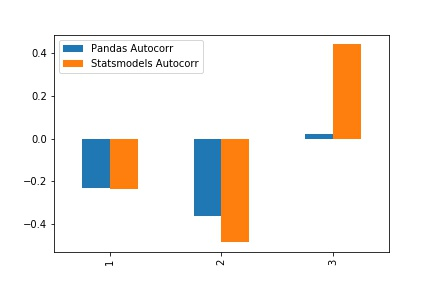
\includegraphics[scale=0.6]{corr_comparison.jpg}
\end{center}

\vspace{5mm}

\underline{Partial autocorrelation}

\vspace{5mm}

Based on article \href{https://towardsdatascience.com/understanding-partial-auto-correlation-fa39271146ac}{understanding-partial-auto-correlation (towardsdatascience)}

\vspace{5mm}

\begin{center}
$PR_k = \frac{cov(X_t | X_{t-1} ... X_{t-k+1},X_{t-k} | X_{t-1} ... X_{t-k+1})}{\sigma_{X_t | X_{t-1} ... X_{t-k+1}} \sigma_{X_{t-k} | X_{t-1} ... X_{t-k+1}}}$
\end{center}

$X_t | X_{t-1} ... X_{t-k+1}$ is the residual of regression $X_t = \beta_0 + \beta_1 X_{t-1} + ... + \beta_k X_{t-k+1}$

$X_{t-k} | X_{t-1} ... X_{t-k+1}$ is the residual of regression $X_{t-k} = \beta_0 + \beta_1 X_{t-1} + ... + \beta_k X_{t-k+1}$

\vspace{5mm}

Thus, one can write:

\begin{center}
$PR_k = \rho_{\epsilon_t,\epsilon_{t-k}}$
\end{center}

\vspace{5mm}

We use partial autocorrelation in order to define the order $p$ in which we can compute an AR(p) model.

\begin{center}
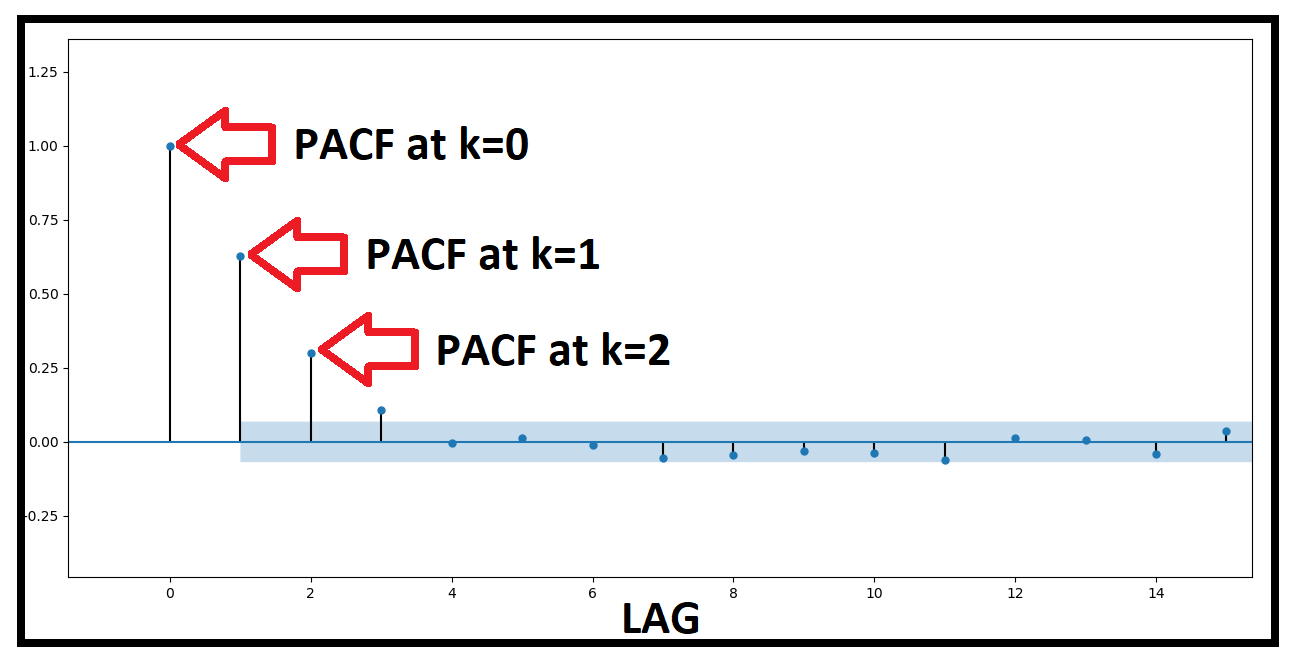
\includegraphics[scale=0.2]{PACF.png}
\end{center}

\vspace{5mm}

Based on this graph, we can use an AR(2) or even AR(3) ($k=3$ is just outside the 95\% confidence interval.

\vspace{5mm}

{\fontsize{12pt}{22pt} \textbf{Time series}\par}

\vspace{5mm}

\underline{Differential equations}

\vspace{5mm}

A differential equation is an equation with the following characteristics:

- variables = functions

- it expresses the relationship of functions (variables) with their derivatives

\vspace{5mm}

Case of \textit{linear and constant coefficient} differential equations:

\vspace{5mm}

\begin{center}
$a_ny^{(n)} + a_{n-1}y^{(n-1)} + ... + a_1y' + a_0y = 0$  (E)
\end{center}

$(n)$: n-th derivative

\vspace{5mm}

In order to solve such equations, we use \textit{characteristic equations}. Let $y(x) = e^{rx}$

(E) => $a_nr^n e^{rx} + a_{n-1}r^{(n-1)} e^{rx} + ... + a_1 r e^{rx} + a_0e^{rx} = 0$

Since $e^{rx} \neq 0$

(E) => $a_nr^n + a_{n-1}r^{(n-1)} + ... + a_1 r + a_0 = 0$

We thus end up with a polynomial function.

In order to find the general solution of (E), we can find the solution of the characteristic equation and deduce the general solution (using exponential).

\vspace{5mm}

\underline{Autoregressive processes}

\vspace{5mm}

Autoregressive processes are a specifc case of \textit{differential equations}.

\vspace{5mm}

$y_{t+k} = \beta_1 y_{t+k-1} + \beta_2 y_{t+k-2} + ... + \beta_k y_{t}$

\vspace{5mm}

Characteristic equation:

$r^k - \beta_1 r^{k-1} - ... - \beta_{k-1} r - \beta_k = 0$

\vspace{5mm}

\underline{Stationary processes}

\vspace{5mm}

A stationary process has the same moment (expectation, variance, etc.)  in every single point.

In practice, we check the stationarity with only the first two moments (expectation and variance).

\vspace{5mm}

Intuition behind the importance of stationary processes in regressions:

When performing regressions, it is important to make sure the error term is stationary. If non stationary, there's probably a trend that is not caught by the explanatory variables used. This can lead to \textit{spurious regressions}.

\vspace{5mm}

To make sure a process is stationary, we have to check the existence of a \textit{unit root}.

\vspace{5mm}

Why existence of unit root leads to non-stationary process?

Toy example:

Let us consider a 1st order autoregressive process $y_t = \beta_0 + \beta_1 y_{t-1} + \epsilon_t$

Let $\beta_0 = 0$. The characteristic equation is:

$r - \beta_1 = 0$

The solution is $r = \beta_1$

The problem has thus a unit root when $\beta_1 = 1$

Since $y_t = \beta_0 + \beta_1 y_{t-1} + \epsilon_t$ we can write:

$y_1 = y_0 + \epsilon_0$

$y_2 = y_1 + \epsilon_1 = y_0 + \epsilon_0 + \epsilon_1$

$y_3 = y_0 + \epsilon_0 + \epsilon_1 + \epsilon_2$

Thus, $y_t = y_0 + \Sigma_{j=0}^t \epsilon_j$

The variance is $\mathbb{V}[y_t] = t \sigma^2$ (we assume a constant variance for $\epsilon$)

Consequently, the variance is increasing with time so the process is \textbf{not stationary}.

\vspace{5mm}

To detect stationarity, we can perform a unit root test such as \textit{Augmented Dicky Fuller test}.

\vspace{5mm}

Non stationarity can be corrected in several ways :

- time regression : performing a regression on time and working with the error term

Example : if $y_t$ in non stationary

$y_t = \beta_0 + \beta_1 t +\epsilon_t$ --> $\epsilon_t$ will not depend on time anymore

- finite differences : removing previous term to each observation $y_t = y_t - y_{t-1}$ --> this will have the effect to remove the trend

- moving average NxN

Example : using (double) centered moving average 5x5 

\lstset{language=Python}
\lstset{frame=lines}
\lstset{caption={Centered moving average (double)}}
\lstset{label={lst:code_direct}}
\lstset{basicstyle=\footnotesize}
\begin{lstlisting}

cpi_roll = cpi.rolling(window=5).mean() # cell at index 4 is the mean of the 5 previous ones (inclusive)
cpi_mm = cpi - cpi_roll
cpi_roll_2 = cpi_mm.rolling(window=5).mean()
cpi_mm_2 = cpi_mm - cpi_roll_2

\end{lstlisting}

\vspace{5mm}
{\fontsize{12pt}{22pt} \textbf{Heavy-Tailed Distribution}\par}

\vspace{5mm}

A distribution is heavy-tailed when there are more chances to get large values. Consequently, the variance is higher and will make the mean misleading as many outliers have high values. Below are p.d.f. (light-tailed and heavy-tailed):

\vspace{5mm}

\begin{center}
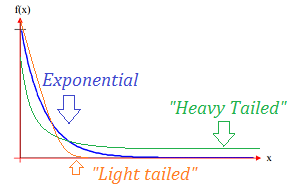
\includegraphics[scale=0.8]{heavy-light-tailed.png}
\end{center}

A real-life example of heavy-tailed distribution is the income in the US.

\vspace{5mm}
{\fontsize{12pt}{22pt} \textbf{Central Limit Theorem}\par}

\vspace{5mm}

Let $(X_n)_{n \ge 1}$ be a real and independent sequence with same law such that $\mu = \mathbb{E}[X_1]$ and \\
$\mathbb{V}[X_1]=\sigma^2$ are defined ($\mathbb{V}[X_1] \leq +\infty$). Noting $\bar{X}_n=\frac{1}{n}(X_1 + ... + X_n)$, we have:
\begin{center}
$\sqrt{n}\frac{(\bar{X}_n-\mu)}{\sigma} \sim_{n \to \infty} \mathcal{N}(0,1)$
\end{center}

\vspace{5mm}
{\fontsize{12pt}{22pt} \textbf{Spectral Theorem}\par}

\vspace{5mm}

Let $M$ be a symmetric matrix with real coefficients. Then it exists $U$ orthogonal and $D$ diagonal with real coefficients such that $M=UDU^T$.

\vspace{5mm}
{\fontsize{20pt}{22pt}\selectfont \textbf{Inferential statistics} \par}
\vspace{10mm}
{\fontsize{12pt}{22pt} \textbf{Parametric Tests}\par}

\vspace{5mm}

A test is \textit{parametric} if its goal is to test parameters of a known/unknown distribution. \\

Note: we call \textit{population} the total data from which a \textit{sample} is extracted. A statistical test aims at finding information about the distribution the sample is extracted from.

\vspace{5mm}

Procedure:

1) find the test to perform

2) find the right estimator to use

3) deduce the reject region

4) compute the test statistic

5) retrieve quantiles of known distributions

\vspace{5mm}

See the \href{https://github.com/savoga/various_projects/blob/master/statistical_testing.ipynb}{associated notebook} for numerical examples.

\vspace{5mm}

Example 1 \textbf{(\textbf{Z-test})}: 

\vspace{5mm}

(\textit{inspired from example in Saporta p.325})

\vspace{5mm}

$X_1,...,X_n~(iid)\sim \mathbb{P_\theta}$

\vspace{5mm}

We want to know the mean of an unknown distribution from which we have a sample. \\

Requirements/assumptions:

- we need the standard deviation of the population \\
    
Note: there is no assumption on the unknown distribution law (if the random variable is not Gaussian, we can still use the CLT to have the normality).

\vspace{5mm}

1) find the test to perform

\vspace{5mm}

$
\left\{
    \begin{array}{ll}
        \mathcal{H}_0: m=a \\
        \mathcal{H}_1: m>a \\
    \end{array}
\right.
$

\vspace{5mm}

2) find the right estimator to use

\vspace{5mm}

Since we are testing the mean, we choose the empirical mean as \textbf{estimator} $\widehat{\theta}=\frac{1}{n}\sum{X_i}$

\vspace{5mm}

3) deduce the reject region

\vspace{5mm}

We fix $k$ for a rejection level $\alpha$. The rejection region is:

$Z=\{\widehat{\theta} \ge k\}$

\vspace{5mm}

We look for $k$ defined as such:

$\mathbb{P}_{\theta \in \Theta_0}(\widehat{\theta} \ge k)=\alpha$ => under $\mathcal{H}_0$, we reject the hypothesis when our estimator $\widehat{\theta}$ is above $k$

\textit{Intuitively, we want to keep our hypothesis if it's verified in most of the cases => under our hypothesis, there is a low probability that we are in the rejection region.}

\textit{Thus, if in real life we have a result that makes the hypothesis unverified, we reject the hypothesis. However, we have a risk of $\alpha$ that our hypothesis was correct and that we ended up in the rejection region by mistake.}

\vspace{5mm}

4) compute the test statistic

\vspace{5mm}

We center and reduce the estimator in order to get the Gaussian law and thus end up with known quantiles:

$\mathbb{P}_{\theta = a}(T \ge \frac{\sqrt{n} (k-a)}{\sqrt{\sigma^2}})=\alpha$ with $T \sim_{n \to \infty} \mathcal{N}(0,1)$

$T$ is the test statistic (\textcolor{red}{a test statistic is a random variable for which we know the law under $\mathcal{H}_0$})

\vspace{5mm}

5) retrieve quantiles of known distributions

\vspace{5mm}

Finally, $\frac{\sqrt{n} (k-a)}{\sqrt{\sigma^2}}=q_\alpha$ => we can find $k$ telling us when rejecting $\mathcal{H}_0$

\vspace{5mm}

$\alpha$ is also called the p-value. The lower the p-value is, the less error we make in rejecting our hypothesis so the more significant the rejection is.

\textcolor{red}{p-value is the lowest error probability we want to make when rejecting our hypothesis.}

\vspace{5mm}

When performing OLS, our hypothesis is $\theta_{x1}=0$ so we don't reject it if the pvalue column is higher than our threshold. In the below OLS result, pvalues are displayed in column $P>|t|$. All variables are significant.

\begin{center}
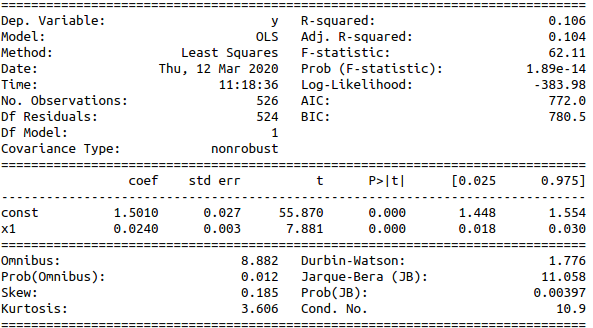
\includegraphics[scale=0.5]{OLS_pvalue.png}
\end{center}

Example 2 (\textbf{T-test}):  when the variance is not known.

\vspace{5mm}

Say we want to test whether a coefficient is zero:

1) find the test to perform

\vspace{5mm}

$
\left\{
    \begin{array}{ll}
        \mathcal{H}_0: \theta_j=0 \\
        \mathcal{H}_1: \theta_j \neq 0 \\
    \end{array}
\right.
$

\vspace{5mm}

2) find the right estimator to use

\vspace{5mm}

$\widehat{\theta_j} = (X^TX)^{-1}X^TY$

\vspace{5mm}

3) deduce the reject region

\vspace{5mm}

$Z=\{k_1 \leq \widehat{\theta_j} \leq k_2\}$

\vspace{5mm}

4) compute the test statistic

\vspace{5mm}

$T_j = \frac{\widehat{\theta_j}-\theta_j}{\sigma_{\theta_j}} = \frac{\widehat{\theta_j}}{\sigma_{\theta_j}}  \sim \mathcal{N}(0,1)$ with $\sigma_{\theta_j} = \sigma \sqrt{(X^TX)^{-1}}$ (recall that $\sigma = \sigma_{\epsilon}$)

\vspace{5mm}

Since we don't know $\sigma$, we can use the Cochrane theorem to remove this value:

$T_j = \frac{ \frac{\widehat{\theta_j}}{\sigma \sqrt{(X^TX)^{-1}}} \sim \mathcal{N}(0,1)}{\sqrt{\frac{\widehat{\sigma}^2 (n-p-1)}{\sigma^2} \sim \mathcal{X}_{n-p-1}}} \sim \mathcal{T}(n-p-1)$ with $\widehat{\sigma}^2 = \frac{1}{n-p-1} \Sigma \epsilon ^2$

$ T_j = \frac{\widehat{\theta_j}}{\Sigma \epsilon ^2 \sqrt{(X^TX)^{-1}}}$

\vspace{5mm}

5) retrieve quantiles of known distributions

\vspace{5mm}

Finally,


$\mathcal{P}_{\theta_j=0}(\frac{k_1}{\Sigma \epsilon ^2 \sqrt{(X^TX)^{-1}}} \leq T_j \leq \frac{k_2}{\Sigma \epsilon ^2 \sqrt{(X^TX)^{-1}}}) = \alpha$

Thus, $\frac{k_1}{\Sigma \epsilon ^2 \sqrt{(X^TX)^{-1}}} = t_{\frac{\alpha}{2}}$ (same for $k_2$)

\vspace{5mm}

Example 3 (\textbf{T-test} with forward selection):

\vspace{5mm}

Concept: 

Regress all variables one by one on the most significant variable's residual, remove the most significant variable after each full round

\vspace{20mm}

\begin{algorithm}
\caption{Forward selection}
\begin{algorithmic}
\State $sel \_ variables \leftarrow \emptyset$
\For{$i=1$ to $nb \_variables$}
\State $resid \_mem \leftarrow \emptyset$
\State $T \_stats \leftarrow \emptyset$
\For{$j=1$ to $rem \_ variables$}
\State $Y = X_j\theta$
\State $resid \_mem \leftarrow resid \_mem + \{res\}$ // adding residuals from previous regression
\State $T \_ stats \leftarrow T \_stats + \{T_j\}$ // $T_j$ is computed as seen in example 2
\EndFor
\State $k \leftarrow argmax(T \_ stats)$
\State $Y = resid \_ mem (k)$
\State $rem \_ variable \leftarrow rem \_ variable - \{k\}$
\State $sel \_ variables \leftarrow sel \_ variables + \{k\}$
\EndFor
\end{algorithmic}
\end{algorithm}

\begin{center}
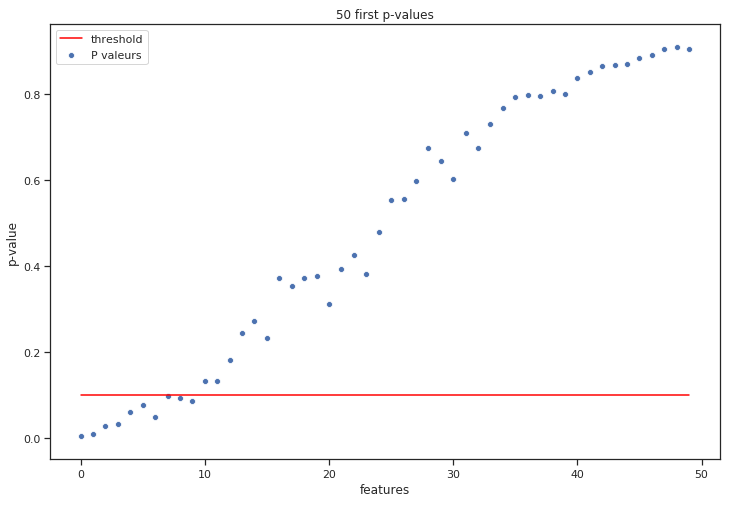
\includegraphics[scale=0.5]{forward_sel_pval.png}
\end{center}

(x-axis is the order in which we selected variables; see notebook \textit{ACP\_ForwardSelection\_Ridge\_Lasso.ipynb})

We can then select only the most significant variables based on p-values on variables from list $sel \_ variables$

\textit{Note}: since $pval = 2*(1-cdf(T)) = 2*\frac{1-(1-\alpha)}{2}$, choosing the biggest T-stat is equivalent to choose the smallest p-value

\vspace{5mm}

Example 4 (\textbf{F-test}):

\vspace{5mm}

When several variables are correlated (often the case in practice), the student test is not efficient enough since it does not take the correlation into account. F-test allows to test \textbf{global} significativity.

Let's say we have 4 variables and we want to check the significativity of 2 of them.

\vspace{5mm}

$
\left\{
    \begin{array}{ll}
        \mathcal{H}_0: \theta_1 = \theta_2 = 0\\
        \mathcal{H}_1: \theta_1, \theta_2 \neq 0 \\
    \end{array}
\right.
$

\vspace{5mm}

$SSR = sum~squared~residuals = \Sigma (\widehat{y_i} - y_i)^2$

\vspace{5mm}

$F = \frac{(SSR_C - SSR_{NC})/(p_{NC} - p_C)}{(SSR_{NC})/(n-p_{NC})} \sim \mathcal{F}(p_{NC} - p_C, n-p_{NC})$

\vspace{5mm}

NC: not constraint model

C: constraint model

\vspace{5mm}

Method:

- OLS on not constraint model => computation of $SSR_{NC}$

- OLS  on constraint model => computation of $SSR_{C}$

- Computation of the Fisher stat => computation of p-value (using complementary cumulative distribution function as above)

\lstset{language=Python}
\lstset{frame=lines}
\lstset{caption={F-test}}
\lstset{label={lst:code_direct}}
\lstset{basicstyle=\footnotesize}
\begin{lstlisting}

# Non constraint model
X0=np.column_stack((educ, exper, tenure, const))
model=sm.OLS(y,X0)
results = model.fit()
u=results.resid
SSR0=u.T@u

# Constraint model
X=np.column_stack((const, educ, tenure))
model=sm.OLS(y,X)
results = model.fit()
u=results.resid
SSR1=u.T@u

# Computation of Fisher stat
n=np.shape(X0)[0]
F=((SSR1-SSR0)/1)/(SSR0/(n-4))
f.sf(F,1,n-4) # p-value

\end{lstlisting}


\vspace{5mm}
{\fontsize{12pt}{22pt} \textbf{Non-Parametric Tests}\par}

\vspace{5mm}

Example 1 \textbf{(Kolmogorov-Smirnov test)}: 

\vspace{5mm}

- Test whether a sample follow a known law \\

$F$ is the cumulative ditribution function and $\widehat{F_n}$ its empirical estimation. \\

The statistic test is $\widehat{F_n}(x) - F(x)$. \\

We have, \\

$\sqrt{n} \underset{1 \leq i \leq k}{\operatorname{max}}|\widehat{F_n}(x_i) - F(x_i)| \underset{n \rightarrow + \infty}{\rightarrow} \underset{0 \leq i \leq k}{\operatorname{max}}|W_i|$ where $W_i$ is a \textit{Brownian motion} or \textit{Wiener process}.\\

We also have, \\

$\sqrt{n} \underset{0 \leq x \leq 1}{\operatorname{max}}|\widehat{F_n}(x) -x)| \underset{n \rightarrow + \infty}{\rightarrow} \underset{0 \leq x \leq 1}{\operatorname{max}}|B(x)|$ where $B$ is a \textit{Brownian bridge}.\\

\href{http://www.math.utah.edu/~davar/ps-pdf-files/Kolmogorov-Smirnov.pdf}{Proofs (Empirical-Process Theory)} \\

A Brownian bridge has the following property: \\

$\mathbb{P}(\underset{t \in [0,1]}{\operatorname{sup}}|B_t| \geq b) = 2 \Sigma_{n \geq 1}(-1)^{n-1}e^{-2n^2b^2}$.

This allowed statisticians to draw a quantile table, we can thus easily know the critical region.

\vspace{5mm}

- Test whether two samples follow the same law \\

In that case, the statistic is the distance $D_{n,m} = sup_x |\widehat{F}_{1,n}(x) - \widehat{F}_{2,m}(x)|$. \\

Associated test hypothesis are: \\

$
\left\{
    \begin{array}{ll}
        \mathcal{H}_0: \widehat{F}_{1,n}(x) = \widehat{F}_{2,m}(x) \\
        \mathcal{H}_1: \widehat{F}_{1,n}(x) \neq \widehat{F}_{2,m}(x) \\
    \end{array}
\right.
$

We reject the null hypothesis for level $\alpha$ if $D_{n,m} > \frac{1}{\sqrt{n}} \sqrt{-ln(\frac{\alpha}{2}) \frac{1 + \frac{n}{m}}{2}}$. \\

\textit{Scipy} \\

\underline{Test statistic computation}

\lstset{language=Python}
\lstset{frame=lines}
\lstset{caption={Kolmogorov-Smirnov test statistic}}
\lstset{label={lst:code_direct}}
\lstset{basicstyle=\footnotesize}
\begin{lstlisting}

cdf1 = np.searchsorted(data1, data_all, side='right') / n1
cdf2 = np.searchsorted(data2, data_all, side='right') / n2
cddiffs = cdf1 - cdf2
T = np.max(cddiffs)

\end{lstlisting}

\underline{Critical probability computation} \\

The critical probability is computed differently depending on sample size. If sample size is small, an exact computation is done. If sample size is large, an asymptotic computation is done.
In both cases, the critical probability is computed using combinatorics and largely inspired by \href{https://projecteuclid.org/download/pdf_1/euclid.afm/1485893310}{J. L. Hodges, Jr.}.

\vspace{5mm}

Example 2 \textbf{(Wilcoxon-Mann-Whitney test} or \textbf{Mann-Whitney U test)}: 

\vspace{5mm}

- Test whether two samples follow the same law \\

$
\left\{
    \begin{array}{ll}
        \mathcal{H}_0: \widehat{F}_{1,n}(x) = \widehat{F}_{2,m}(x) \\
        \mathcal{H}_1: \widehat{F}_{1,n}(x) \neq \widehat{F}_{2,m}(x) \\
    \end{array}
\right.
$

\vspace{5mm}

The test statistic is $U = \Sigma rank_1 - \frac{n_1(n_1+1)}{2}$ where $rank_1$ are the ranks of each element from the first dataset in the second dataset. \\

\underline{Intuition behind the test}

The test is equivalent of ranking all elements from the two datasets; if the resulting dataset is well mixed, the p-value is likely to be high (similar distributions).

The test can also be interpreted as a comparison between the two medians; if they are very different, distributions are likely to be different.

\vspace{5mm}

Example 3 \textbf{(Fisher exact test)}: 

\vspace{5mm}

- Test whether proportions are representative \\

$\mathcal{H}_0: \text{proportions are representative} $ \\

This test is to be used for the analysis of contingency tables.

\begin{center}
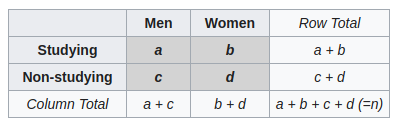
\includegraphics[scale=0.6]{fisher_contingency_table.png}
\end{center}

Fisher showed that knowing the total numbers (Row Total and Column Total), the probability to have a certain combination follows a \textit{hypergeometric} distribution.

$$p = \frac{C_a^{a+b} C_c^{c+d}}{C_{a+c}^n}$$

The test is said \textit{exact} since there is no asymptotic behavior in the formula. \\

$p < \alpha$ means that, based on total numbers, this specific combination is unlikely to happen.

\vspace{5mm}
\vspace{10mm}
\vspace{10mm}
{\fontsize{12pt}{22pt} \textbf{Likelihood method}\par}

\vspace{5mm}

This method consists on finding the parameter that maximizes the likelihood of an event. The event here is to observe some data. It is usually done when we know the type of law of a random variable (uniform, gaussian etc.) and we are looking for the parameter that maximizes the likelihood ($\approx$ probability) that an event occurs.

\vspace{5mm}

$L(\theta; x_1,...,x_n) = \prod_{i=1}^{n}f(x_i;\theta)$ which is the product of densities across all samples.

In discrete form: $L(\theta; x_1,...,x_n) = \prod_{i=1}^{n}\mathbb{P}(X = x_i; \theta)$


\vspace{5mm}

\textit{Note (wording clarification)}: $L(\theta | X) = \mathbb{P} (X | \theta)$

$\mathbb{P} (X | \theta)$: the probability of observing an event with fixed model parameters.

$L(\theta | X)$: the likelihood of the parameters taking certain values given that we observe an event.

\vspace{5mm}

Intuitively, we want to find the $\theta$ that maximizes a certain event, that is, \textbf{obtaining some data $X$} (which is why we have $X | \theta$).

We often use the log in order to get rid of power coefficients appearing with the product. \\
\textit{likelihood equation}: $\frac{d}{d\theta}ln(L(x_1,...,x_n;\theta))=0$

\vspace{5mm}

\textit{Note}: in machine learning, we use likelihood maximization in unsupervised learning when we want to estimate parameters of a distribution sample (generative models).

\vspace{5mm}
{\fontsize{20pt}{22pt}\selectfont \textbf{Exploratory statistics} \par}
\vspace{10mm}
{\fontsize{12pt}{22pt} \textbf{Distance Metrics}\par}

\vspace{5mm}

In statistic, the generic distance metric is expressed as follow:

$$d(x,y)=(x-y)^TM(x-y)$$

where $M$ is a symmetric positive definite matrix. \\

\textit{Note}: the distance is a number (1 dimension). \\

\underline{Euclidean distance} \\

This is equivalent to the generic definition with $M=Id$. \\

Euclidean distance is also called the 2-norm: $\Sigma_{i=1}^n (x_i - y_i)^2$ \\

\underline{Mahalanobis distance} \\

This is equivalent to the generic definition with $M=\Sigma^{-1}$. \\

It is also common to define the squared distance between a vector $x$ and its mean vector $\mu_x$:

$$D^2=(x-\mu_x)^T\Sigma^{-1}(x-\mu_x)$$

Advantage : it takes into account the data standard deviation and correlation. The more the data is dispersed, the lower the distance is. Indeed, using the inverse matrix is like if we divided the distance from the mean $(x-\mu_X)$ by the standard deviation.


\vspace{5mm}
{\fontsize{12pt}{22pt} \textbf{Principal component Analysis}\par}

\vspace{5mm}

The PCA's objective is to get an approximation of a set of points in a \textbf{low} dimensional set. \\

\underline{Inertia} \\

Inertia $I_g = \Sigma_{i=1}^n p_i ||x_i - g||_M^2$ \\

where $g^T = (\bar{x}^{(1)},...,\bar{x}^{(p)})$ also called the \textit{gravity center}. \\

--> The inertia is thus the weighted average of the squared distance of each observation with the gravity center. \\

--> $p_i$ is the weight given to each observation. Most of the times, $p_i = \frac{1}{n}$ (every observation contributes equally to the analysis) \\

-->  the distance $||.||$ depends on the choosen metric $M$ \\

\underline{Projection} \\

In order to represent the set of points in a low dimensional set, we use projections. \\

The projection should distort the initial set the less as possible, that is:

=> reduce the projection distances as much as possible

=> maximize the average of squared distances between projected points

=> maximize inertia of the projected points \\

In the below figure, maximizing the inertia leads to choosing the projection on the right since d2 > d1.

\begin{center}
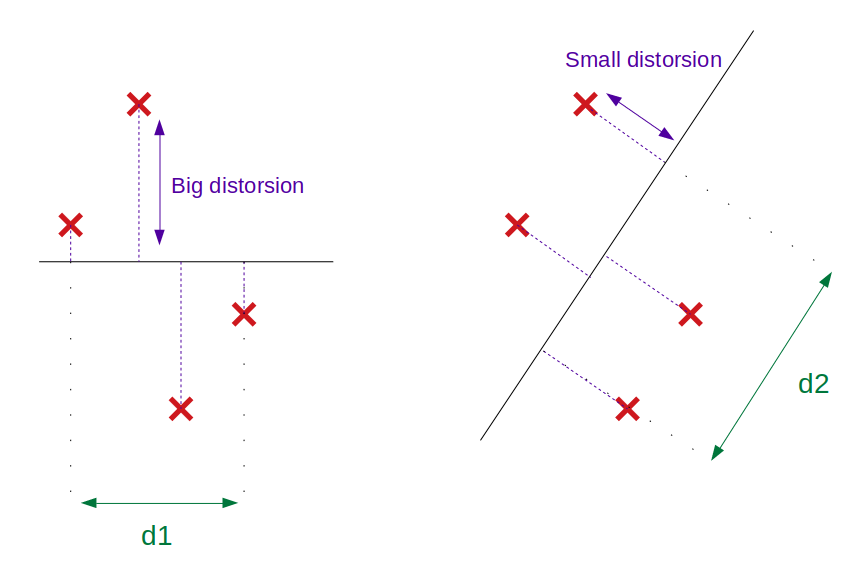
\includegraphics[scale=0.4]{PCA_projections.png}
\end{center}

\underline{Optimisation} \\

If the data are centered, we can also write $I_g = \Sigma_{i=1}^n p_i x_i^T M x_i$ \\

Exprimer l'inertie en fonction de la matrice de covariance.

Exprimer la matrice de covariance du nuage de points projetés.

Exprimer l'inertie en fonction de la matrice de covariance projetés.

Maximiser l'inertie...

\vspace{5mm}
\vspace{10mm}
{\fontsize{20pt}{22pt}\selectfont \textbf{Predictive models} \par}
\vspace{10mm}
{\fontsize{12pt}{22pt} \textbf{Linear regression}\par}

$$Y = X \theta + \epsilon$$

Hypothesis: $
\left\{
    \begin{array}{ll}
        \mathbb{E}[\epsilon] = 0 \\
        \mathbb{V}[\epsilon] = \sigma
    \end{array}
\right.
$ \\

\underline{Bias}

$$Bias = \mathbb{E}[\widehat{\theta}-\theta^*]$$

\begin{align*}
  \mathbb{E}[\widehat{\theta}] &= \mathbb{E}[(X^TX)^{-1}X^TY] \\
            &= \mathbb{E}[(X^TX)^{-1}X^T(X \theta^* + \epsilon)] \\
	   &= \theta^* + (X^TX)^{-1}X^T\mathbb{E}[\epsilon] \\
	   &= \theta^*
\end{align*}

The estimator is \textbf{not biased}. \\

\underline{Variance-covariance}

\begin{align*}
  Cov(\widehat{\theta}) &= \mathbb{V}[(X^TX)^{-1}X^TY] \\
            &= \mathbb{V}[(X^TX)^{-1}X^T(X \theta^* + \epsilon)] \\
	   &= 0 + ((X^TX)^{-1}X^T)^T\mathbb{V}[\epsilon] (X^TX)^{-1}X^T \\
	   &= (X^TX)^{-1}\sigma^2 ~~~~\text{ since $X^TX$ is symmetric}
\end{align*}

\textit{Note}: the variance-covariance is a matrix. We define here the variance as a number. \\

$\mathbb{V}[\widehat{\theta}] = \mathbb{E}[(\widehat{\theta} - \mathbb{E}[\widehat{\theta}])^2]$ \\

We know that $||u||_2 = \Sigma_k u_k^2 = Tr(u u^T)$. \\

Thus:

\begin{align*}
\mathbb{V}[\widehat{\theta}] &= \mathbb{E}[Tr((\widehat{\theta} - \mathbb{E}[\widehat{\theta}])(\widehat{\theta} - \mathbb{E}[\widehat{\theta}])^T)] \\
	&= Tr(\mathbb{E}[(\widehat{\theta} - \mathbb{E}[\widehat{\theta}])(\widehat{\theta} - \mathbb{E}[\widehat{\theta}])^T)] ~~~ \text{ since the trace is a number} \\
	&= Tr(Cov(\widehat{\theta})) \\
	&= Tr((X^TX)^{-1}\sigma^2) \\
	&= \sigma^2Tr((UDU^T)^{-1}) ~~~ \text{ thanks to the spectral theorem (we assume inversible matrices)} \\
	&= \sigma^2Tr((UU^T)^{-1}D^{-1}) ~~~ \text{ thanks to the trace properties} \\
	&= \sigma^2Tr(D^{-1}) ~~~ \text{ since $U$ is orthogonal} \\
	&= \sigma^2Tr(\begin{bmatrix}\frac{1}{\lambda_1} & \dots & 0 \\ \vdots & \ddots & \vdots \\ 0 & \dots & \frac{1}{\lambda_p}\end{bmatrix})~~~ \text{with $\lambda_i$ the eigenvalues}  \\
	&= \sigma^2\Sigma_{k=1}^p \frac{1}{\lambda_k}
\end{align*}

We can see that the variance becomes \textbf{unstable} when eigenvalues are small, which is the case when variables are collinear.

\vspace{5mm}

{\fontsize{12pt}{22pt} \textbf{Performance metrics for classification}\par}

\vspace{5mm}

1) ROC = Receiver Operating Curve \\

\underline{Use of the ROC}

\vspace{5mm}

One model:

We use the ROC to evaluate the performance of one classifying model that we can obtain when varying a threshold.

\vspace{5mm}

Several models:

We use the ROC to compare several classifying models in evaluating the area under the curve (AUC) for a range of threshold.

\vspace{5mm}

\underline{Intuition}

\vspace{5mm}

After running the prediction of a specific model, we draw the confusion matrix (actual vs predited) with a certain threshold.

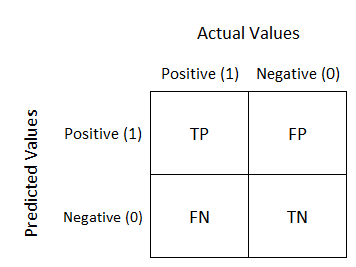
\includegraphics[scale=0.5]{confusionmatrice.png}

\vspace{5mm}

We then modify the threshold and draw another confusion matrix.

The ROC summarizes all of the confusion matrices that each threshold produced.

\vspace{5mm}

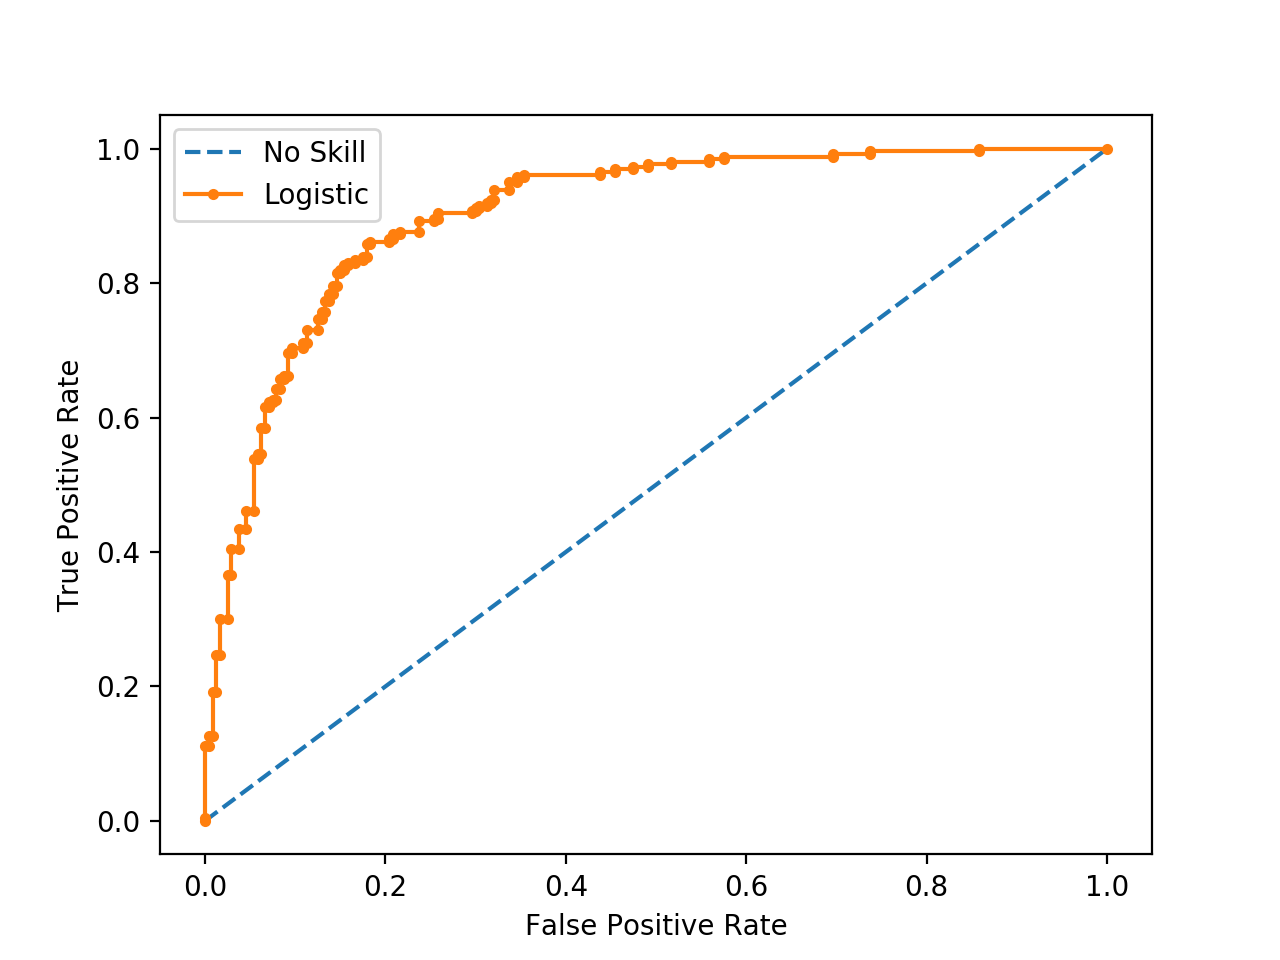
\includegraphics[scale=0.5]{ROC.png}

\vspace{5mm}

The curve is drawn using relationship ratios between predictions and actual results: \\

X-axis: $$FPR = \frac{FP}{N} = \frac{FP}{FP + TN}$$

Y-axis: $$TPR = \frac{TP}{P} = \frac{TP}{TP + FN}$$

\vspace{5mm}

\underline{Implementation}

\vspace{5mm}

1. Get probability predictions

2. Sort the probabilities (prediction)

3. Sort the validation (actual) according to previous sort

4. Loop on the sorted validation. At each iteration:

- increment TP or FP

- compute the TPR and FPR.

5. Plot (FPR, TPR)

\vspace{5mm}

See \textit{https://docs.eyesopen.com/toolkits/cookbook/python/plotting/roc.html} for an implementation example, or data challenge Face\_Recognition. \\

2) PR curve = Precision-Recall curve \\

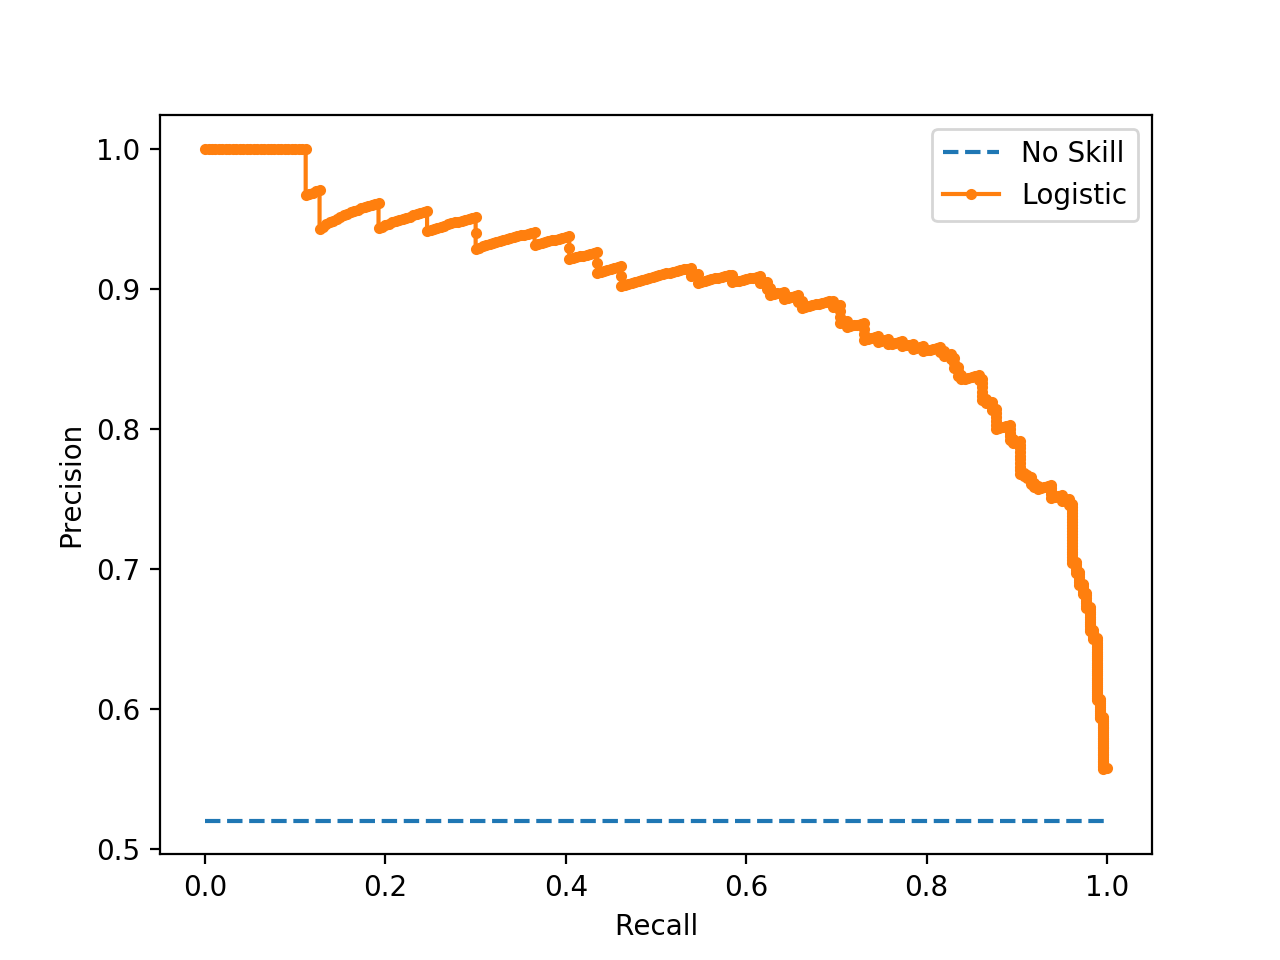
\includegraphics[scale=0.5]{PR_curve.png}

The PR curve uses the following ratios: \\

X-axis:

$$TPR = \text{Recall} = \frac{TP}{P} = \frac{TP}{TP + FN}$$

Y-axis:

$$\text{Precision} = \frac{TP}{TP + FP}$$ \\

The PR curve is better adapted than the ROC in the case of imbalanced data: \\

ROC uses $FPR = \frac{FP}{\textcolor{red}{N}} $ --> $N$ can be either very large or very small if classes are imbalanced.

PR curve uses the $\text{Precision} = \frac{TP}{\textcolor{green}{TP + FP}}$ --> the precision considers only the positive values coming from the model.



\vspace{5mm}

\vspace{10mm}
\end{document} 
